\section{Introduction}

When we project a 3D scene onto a 2D image, there's an inherent ambiguity because different depths can't be distinguished in the image. 
This means that it can be difficult to determine the exact 3D positions of points just from a single image.

However, using multiple views of the same scene can help resolve this ambiguity. 
By taking images from different perspectives, we get different information about the scene that can be used to better understand its 3D structure.
\begin{figure}[H]
    \centering
    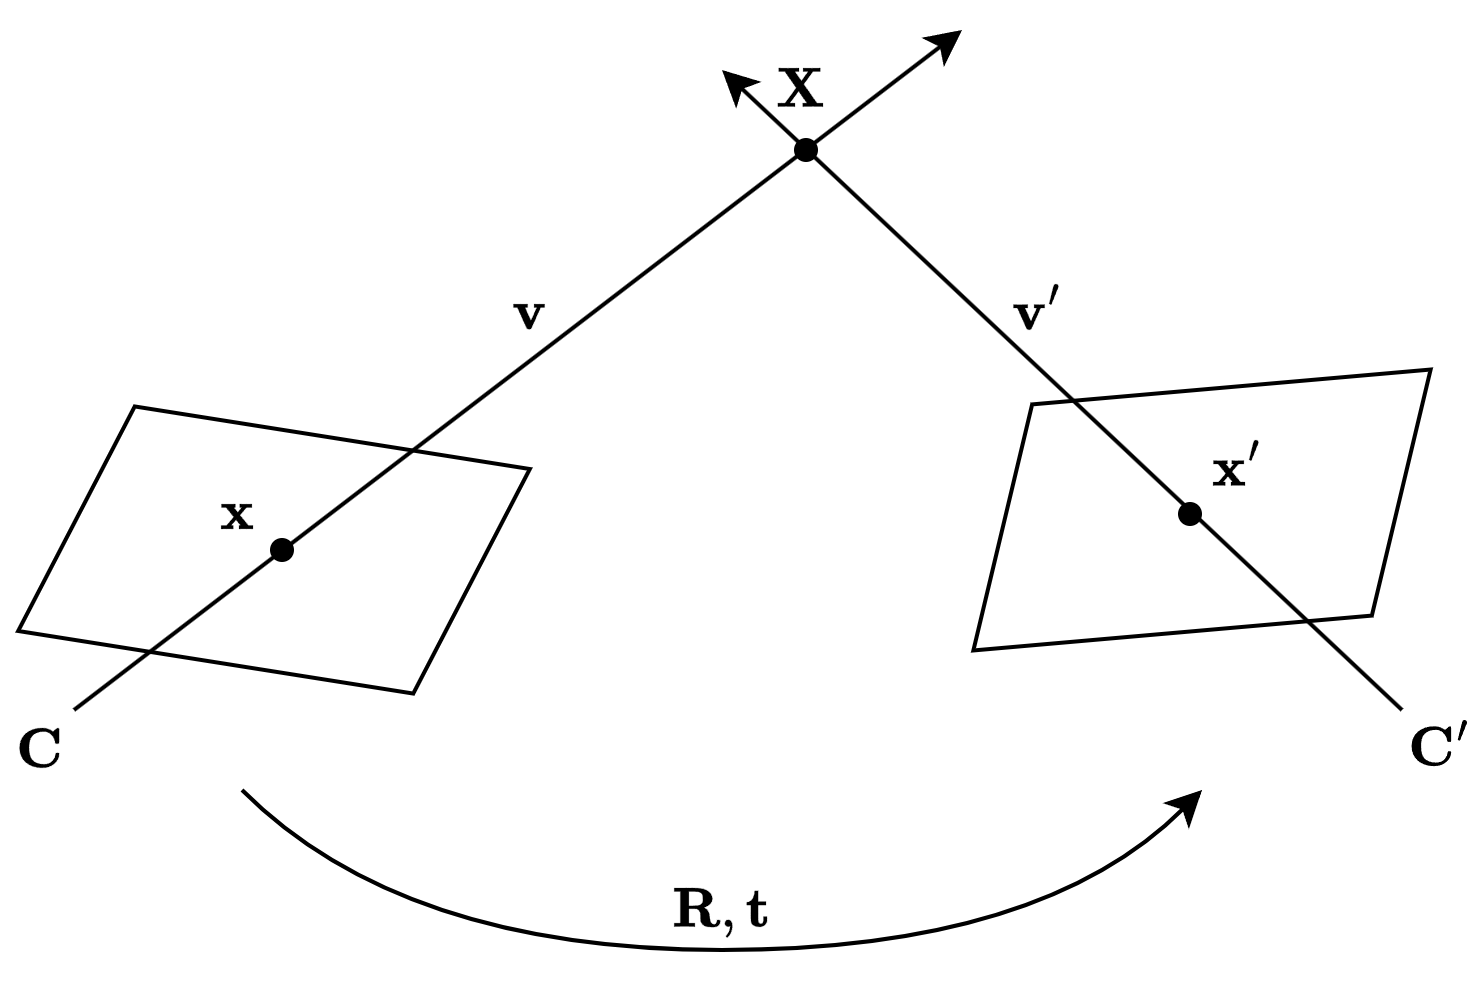
\includegraphics[width=0.5\linewidth]{images/tvg.png}
    \caption{Two view geometry}
\end{figure}

\noindent In a 3D scenario, we can obtain multiple views of a point $\mathbf{X}$ from different cameras, and there are several ways to compute its position:
\begin{itemize}
    \item \textit{Stereo vision}: we know the mapping between the image points $\mathbf{x}$ and $\mathbf{x}^\prime$, as well as the rotation and translation between the two cameras.
        The calibration matrix for both cameras is also known.
        To find the 3D point $\mathbf{X}$, we compute the viewing rays $\mathbf{v}$ or $\mathbf{v}^\prime$ from the calibration matrices $\mathbf{K}$ or $\mathbf{K}^\prime$, and the image points $\mathbf{x}$ or $\mathbf{x}^\prime$. 
        Then, we use triangulation to determine the 3D location:      
        \[\mathbf{X}=\mathbf{v}\cap\mathbf{v}^\prime\]
    \item \textit{Calibrated structure from motion}: we know the mapping between the image points $\mathbf{x}$ and $\mathbf{x}^\prime$, and the calibration matrices for both cameras are known, but the rotation and translation between the two images are unknown.
        To find the 3D point $\mathbf{X}$, as well as the rotation matrix $\mathbb{R}$ and translation vector $\mathbb{t}$, we use the epipolar constraint to estimate $\mathbb{R}$ and $\mathbb{t}$. 
        Afterward, we compute the viewing rays $\mathbf{v}$ and $\mathbf{v}^\prime$ and apply triangulation:
        \[\mathbf{X}=\mathbf{v}\cap\mathbf{v}^\prime\]
    \item \textit{Uncalibrated structure from motion}: we know the mapping between $\mathbf{x}$ to $\mathbf{x}^\prime$, the rotation, translation between the images, and the calibration matrices for the cameras are unknown.
        To estimate the 3D point $\mathbf{X}$, along with the camera calibration matrices $\mathbf{K}$, $\mathbf{K}^\prime$, $\mathbb{R}$, and $\mathbb{t}$, we can use the epipolar constraint and partial information about the scene or cameras.
        Once we have these estimates, we compute the viewing rays $\mathbf{v}$ and $\mathbf{v}^\prime$ and use triangulation:
        \[\mathbf{X}=\mathbf{v}\cap\mathbf{v}^\prime\]
\end{itemize}